\documentclass{article}
\usepackage[utf8]{inputenc}
\usepackage{tikz}
\usepackage{verbatim}

\usepackage[utf8]{inputenc}
\renewcommand{\arraystretch}{1.5}
 

\setlength{\parindent}{0em}
\setlength{\parskip}{1em}

\title{CENNZnet Token Economy}
\author{}
\date{March 2019}

\usepackage{natbib}
\usepackage{graphicx}

\usetikzlibrary{arrows,calc}
\usepackage{relsize}
\newcommand\LM{\ensuremath{\mathit{AS}}}
\newcommand\IS{\ensuremath{\mathit{AD}}}

\begin{document}

\maketitle

\section{Introduction} The paper below proposed describes a novel blockchain economic protocol involving two types of Tokens a Staking Token (\textbf{CENNZ})and a Reward/Expenditure Token (\textbf{CENTRAPAY}) is designed to maintain the latter type at a relatively stabilized value in an elegant way, which promote usage of the main network creating an economic incentive to hold and stake the Staking Token. We aim to stabilize CENTRAPAY in both In-chain Purchasing Power and Off-chain Purchasing Power.

\section{Goal}
Build a model that value of CENTRAPAY is stabilized in terms of \textit{purchasing power}: 

\begin{itemize}
  \item \textit{In-chain Purchasing Power -} \\
  Some certain amount of CENTRAPAY is enough to pay for a standard sized transaction at all time. For simplicity, we assume that fee for a standard transaction is 1 CENTRAPAY in this paper. A different amount of CENTRAPAY will not change the solution.
  \item \textit{Off-chain Purchasing Power - }\\
  1 CENTRAPAY has a relatively stabilized value in terms of CPU and Storage cost for validators, i.e. if a validator sells 1 CENTRAPAY to FIAT, the amount of FIAT they get at different times should be equal to the cost of purchasing some constant units of CPU and Storage at those times. 
\end{itemize}


\section{Model Setup}
In order to have an on chain transaction processed, CENTRAPAY tokens must be acquired to pay the transaction fee. The protocol will burn any CENTRAPAY tokens used in the fee  once the transaction has been processed. The protocol will also mint new CENTRAPAY and distribute to all participating validator nodes as their reward. The protocol can be extended or modified in the future via network approved upgrades, for instance, the allocation of reward proportions for different types of validator nodes could change in the future. 

\begin{itemize}
  \item $t$ - Unit of Time
  
  \item $q$ - Quantity of CENTRAPAY received in a block\\
  $q^{max}$ - Maximum number of CENTRAPAY received in a block.

  \item $b$ - Number of bytes of a standard transaction, e.g. 200 bytes.\\For any user who would like to process a transaction of size $b$, transaction fee of 1 CENTRAPAY is required; and for a transaction of size $\theta\cdot b$, transaction fee of $\theta$ unit of CENTRAPAY is required.
  
  \item $I$ - Mint Multiplier, that system mint $q\cdot I$ unit of CENTRAPAY after receiving transaction fee of $q$ unit of CENTRAPAY. \\
  This is a parameter we could set.
  
  \item $m$ - Number of validators\\
  Suppose for a block produced at time $t$,  $q_t$ unit of CENTRAPAY is received then burnt, then $q_t\cdot I_t$ unit of CENTRAPAY is minted, that each of the $m$ validators receive $q_t\cdot I_t/m$ unit of CENTRAPAY as reward. 
  
  \item  \textbf{\textit{CCC}} - Assume in order to process one more standard transaction of $b$ bytes at time $t$, a validator needs to pay an extra cost for CPU, and we set this cost to be one unit of a new measurement tool that we introduce and name as \textbf{\textit{Current CPU Cost}} (\textbf{$CCC_t$}). \\
  
  Note that \textbf{\textit{as an elegant point in our protocol, valuation of all items, costs and returns can now be measured in unit of CCC}}, avoiding many adjustment issues, e.g. time value of money, cost in fiat currency decreasing in time. On the other hand, it is \textbf{\textit{a user-friendly concept reflecting off-chain purchasing power}}. For instance, for a dApp company operating entirely online, all of its income and expense items can also be measured in $CCC$ that it can easily estimate how much influence using our CENNZ network has on its operation. 
  
  \item $s$ - Assume in order to process one more standard transaction of $b$ bytes at time $t$, a validator needs to pay an extra cost of Storage, which is $s$ times of cost of CPU, i.e. $s$ unit of $CCC_t$.
    
  \item $P$ - Market value of 1 CENTRAPAY in unit of \textbf{$CCC$}, \\
  e.g. $P_t$ represent how many units of $CCC$ 1 CENTRAPAY will be able to purchase at time $t$.

  \item $VC$ - Validator's Variable Cost spent in gaining 1 CENTRAPAY in a block, in unit of $CCC_t$, made of costs spent in CPU and Storage.

  \item $FC$ - Validator's Fixed Cost spent in a block, in unit of $CCC$.\\
  It is a fixed ratio of the variable cost spent in CPU per transaction, written as $k$ unit of $CCC$.

  \item $ATC$ - Validator's Average Total Cost of gaining 1 CENTRAPAY in a block, in unit of $CCC$.
  
  \item $AVC$ - Validator's Average Variable Cost of gaining 1 CENTRAPAY in a block, in unit of $CCC$.
  
  \item $AFC$ - Validator's Average Fixed Cost of gaining 1 CENTRAPAY in a block, in unit of $CCC$.

  
 \end{itemize}

\section{Mint Multiplier}
Now consider a block produced at time $t$, containing $q_t$ standard transactions:\\
After users pay $q_t$ units of CENTRAPAY as the required transaction fee, validators process the block, all CENTRAPAY paid are burnt by the system, and $q_tI_t$ units of CENTRAPAY are minted and distributed to validators as a reward. Cost of the validators are split into Variable Cost and Fixed Cost:

$$q_tI_t\cdot ATC_t=q_t(1+s)m + k\cdot m$$
$$ATC_t=AVC_t + AFC_t$$
$$ATC_t=\frac{(1+s)m}{I_t} + \frac{km/q_t}{I_t}$$

Note that $ATC_t$, the Average Total Cost of gaining 1 CENTRAPAY in a block depends on $q_t$, which vary from 1 to $q^{max}$. One block is produced every four seconds, and we treat an \textit{empty} block containing zero transaction posted by users but only system information as a block containing one standard transaction. $q^{max}$ is the maximum number of standard transactions a block can contain, e.g. 185 estimated according to target network usage. Thus, if we use a fixed Mint Multiplier $I_t$ for all blocks, $ATC_t$ vary significantly for blocks containing different numbers of transactions, as the Average Fixed Cost depends on $q_t$, demonstrated in the following examples using estimated value of parameters $s=1.99$, $k=128$, $m=200$. 

\begin{tabular}{ |p{1cm}|p{2.2cm}|p{5.5cm}|p{1.6cm}|  }
 \hline
 \multicolumn{4}{|c|}{Examples of Estimated $ATC_t$ (in unit of $CCC$)} \\
 \hline
$I_t$&Block Status&Number of Transaction in a Block&$ATC_t$\\
 \hline
1   &\textit{Empty}     &Treating as 1      &26198.00 \\
1   &Quarter Full   &46     &1154.52\\
1   &Half Full  &92     &876.26\\
1   &Full   &185    &736.38\\
 \hline
1.05   &\textit{Empty}     &Treating as 1      &24950.48 \\
1.05   &Quarter Full   &46     &1099.54\\
1.05   &Half Full  &92     &834.53\\
1.05   &Full   &185    &701.31\\
\hline
\end{tabular}

As we can see in the above examples, having a fixed Mint Multiplier for all blocks cause large variance in $ATC_t$, leading fluctuation in supply and market valuation of CENTRAPAY. \par
Instead, if we set our Mint Multipliers wisely for all blocks, we could have a constant $ATC_t$ in unit of $CCC$, which stabilize supply and market valuation of CENTRAPAY. \par

\begin{itemize}

\item For an \textit{empty} block treated as a block with one standard transaction, 
$$ATC^e=\frac{(1+s)m}{I^e} + \frac{km}{I^e}$$

\item For a \textit{full} block with $q_t=q^{max}$, 
$$ATC^f=\frac{(1+s)m}{I^f} + \frac{km/q^{max}}{I^f}$$

\item For an \textit{ordinary} block with $q_t \in [1,q^{max})$, 
$$ATC^{od}=\frac{(1+s)m}{I^{od}} + \frac{km/q_t}{I^{od}}$$

\end{itemize}

We can have
$$ATC^e=ATC^f=ATC^{od} \quad \forall t$$
if we set our Mint Multipliers that, for a preset value of $I^f$ that we set 
$$I^e=I^f \frac{1+s+k}{1+s+ \frac{k}{q^{max}}} \quad and \quad
I^{od}=I^f \frac{1+s+ \frac{k}{q^t}}{1+s+ \frac{k}{q^{max}}} $$

By choosing our Mint Multiplier this way, all validators have the same average total cost in gaining one CENTRAPAY at all time,
$$ATC= \frac{m}{I^f} (1+s+ \frac{k}{q^{max}})$$


\begin{tabular}{ |p{1.7cm}|p{2cm}|p{2cm}|p{1.1cm}|p{2.3cm}|}
 \hline
 \multicolumn{5}{|c|}{Examples of Setting Mint Multiplier Wisely ($I^f$ preset to be 1)} \\
 \hline
$I_t$&Block Status&Number of Transaction in a Block&$ATC_t$ in CCC &Number of CENTRAPAY minted\\
 \hline
$I^e=35.58$   &\textit{Empty}     &Treating as 1      &736.38   &35.58\\
$I^{qf}=1.57$   &Quarter Full   &46     &736.38   &72.12\\
$I^{hf}=1.19$   &Half Full  &92     &736.38   &109.48\\
$I^f=1$   &Full   &185    &736.38   &185\\
 \hline
\end{tabular}

As in the above example, if we preset $I^f$ as 1 (assuming no room for network activity to expand when the block is full so that we do not mint more CENTRAPAY than what we burn), we can calculate the values of Mint Multipliers we should set wisely when a block is \textit{empty}, quarter full and half full. With those strategically chosen $I$, our $ATC_t$ stays constant in all blocks.   

\section{The Market}
Market Demand is the aggregate demand for CENTRAPAY from users of the network: $$Y^{AD}=Q(P)+u$$ affected by \textit{endogenous factor:} market price of CENTRAPAY in $CCC$ as defined earlier, and \textit{exogenous factors:} $u$, an element that encompasses price-independent variations in demand, e.g. $u$ increases as number of active network users grow. \par

Market Supply is the aggregate supply of CENTRAPAY from all validators, that Market Supply curve is the horizontal sum of all individual validators’ supply curves. Note that since all validators supply identical products - CENTRAPAY, with identical constant $ATC$ given we set our Mint Multipliers wisely, they are all price takers of markert price and have horizontal individual supply curves, that the aggregate supply curve is also horizontal. 

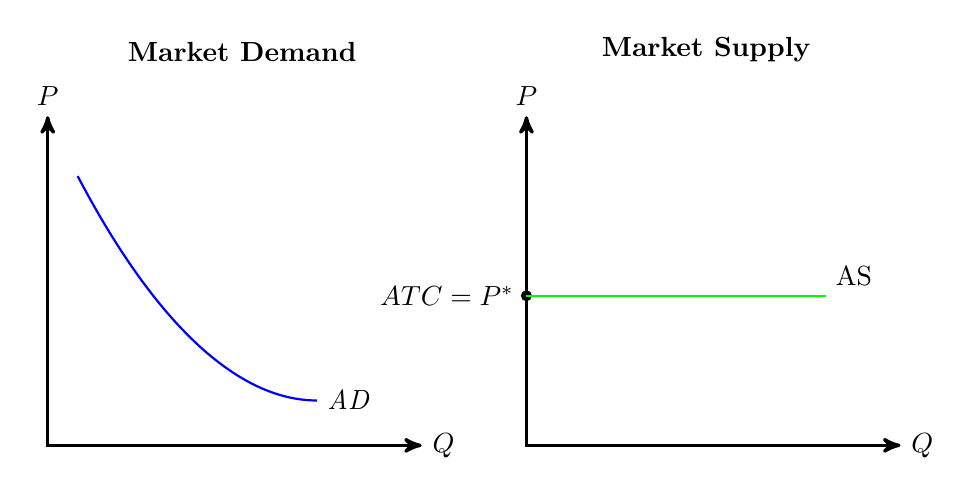
\begin{tikzpicture}[
        scale=1.9,
        IS/.style={blue, thick},
        LM/.style={red, thick},
        axis/.style={very thick, ->, >=stealth', line join=miter},
        important line/.style={thick}, dashed line/.style={dashed, thin},
        every node/.style={color=black},
        dot/.style={circle,fill=black,minimum size=4pt,inner sep=0pt,
            outer sep=-1pt},
    ]

    \draw[axis,<->] (2.5,0) node(xline)[right] {$Q$} -|
                    (0,2.2) 
                    node(yline)[above] {$P$};

    \draw[IS] (0.2,1.8) coordinate (IS_1) parabola[bend at end]
         (1.8,.3) coordinate (IS_2) node[right] {\IS};

    \begin{scope}[xshift=3.2cm]
        \draw[axis,<->] (0,2.2) node(eyline)[above] {$P$} |-
                        (2.5,0) node(exline)[right] {$Q$};
    
        \node[dot,label=left:{$ATC=P^*$}] at (0,1) (int2) {};

        \draw[important line, green, xshift=0cm]
            (0,1) coordinate (es) -- (2,1) coordinate (ee)
            node [above right] {AS};
    \end{scope}

    \coordinate[label= above:\bf{Market Demand}] (p2) at (1.3,2.5) ;  \coordinate[label= above:\bf{Market Supply}] (p4) at (4.4,2.5);
 
\end{tikzpicture}

In the bootstrapping stages, as the whole network is new, users who need to purchase CENTRAPAY to pay for their transaction fees naturally will not have a high valuation for CENTRAPAY  they will not likely pay a price greater or equal to $P^*=ATC$. Instead, for instance, users with demand of $Q_0$ are only willing to purchase CENTRAPAY at price $P_0$ according to their demand curve $AD_0$:  $Y^{AD_0}=Q(P)+u_0$, while $P_0< P*$ that no risk-neutral validators will be willing to sell CENTRAPAY at $P_0$ that their demand of $Q_0$ unit of CENTRAPAY will not be fulfilled fully, which do not encourage growth of the network. \par

Aware of this situation, large CENNZ holders who want to encourage network expansion and risk-takers are willing to sacrifice reduced prices in attempt to encourage usages of the network, by fulfilling all current demand and selling buyers CENTRAPAY at a price lower than their cost of production. For instance, to fulfill demand of $Q_0$, some risk-takers push their own supply curves downwards that the new aggregate supply curve becomes $AS_0$ that the market reaches equilibrium point $B$. \par

As the network and users grow from $u$ to $u_1$ through marketing and development of the network utility, such as getting more dApps to adopt the network, the market demand will build and shift $AD$ curve outwards to $AD_1$, the network will be able to reach a new equilibrium point $C$ where market price $P_1>P_0$ that the risk-taking validators make less loss while the network fulfills more market demand. \par

Similarly, if the network manages to increase $u_1$ to $u_2$ that the $AD$ curve is shifted further outwards to $AD_2$, the network will be able to reach a new equilibrium point $E$ where market price $P^*=ATC$ that all validators reach their break-even points. 

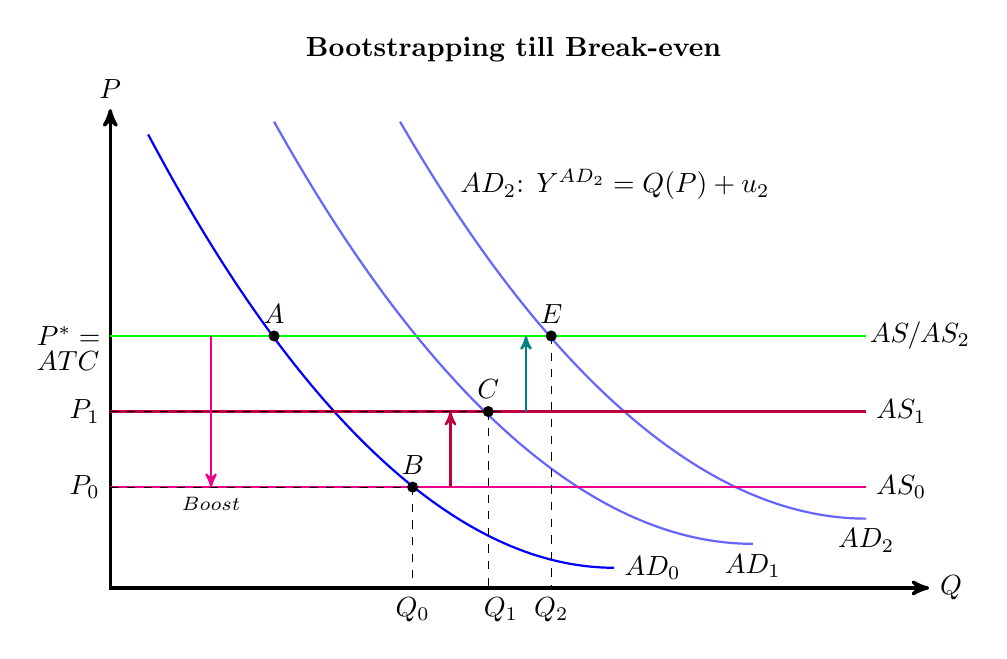
\begin{tikzpicture}[
        scale=1.6,
        IS/.style={blue, thick},
        LM/.style={red, thick},
        axis/.style={very thick, ->, >=stealth', line join=miter},
        important line/.style={thick}, dashed line/.style={dashed, thin},
        every node/.style={color=black},
        dot/.style={circle,fill=black,minimum size=4pt,inner sep=0pt,
            outer sep=-1pt},
    ]

    \draw[axis,<->] (6.5,0) node(xline)[right] {$Q$} -|
                    (0,3.8) 
                    node(yline)[above] {$P$};

    \draw[IS] (0.3,3.6) coordinate (IS_1) parabola[bend at end]
         (4,0.16) coordinate (IS_2) node[right] {$AD_0$};

    \draw[xshift=1cm, yshift=.1cm, IS, blue!60] (0.3,3.6)
        parabola[bend at end]  (4.1,0.25)
        node[below] {$AD_1$};

    \draw[xshift=2cm, yshift=.1cm, IS, blue!60] (0.3,3.6)
        parabola[bend at end]  (4,0.45)
        node[below] {$AD_2$};

    \draw [important line, green] (0,2) -- (6,2);
    \draw [important line, magenta] (0,0.8) -- (6,0.8);
    \draw [important line, purple] (0,1.4) -- (6,1.4);

    \draw [dashed] (0,0.8) -- (2.4,0.8);
    \draw [dashed] (0,1.4) -- (3.1,1.4);

    \coordinate[label= right:{$P^*=$}] (p) at (-0.66,2) ; 
    \coordinate[label= right:{$ATC$}] (atc) at (-0.66,1.8) ; 
    \coordinate[label= right:{$AS/AS_2$}] (as) at (5.95,2) ; 
    \coordinate[label= right:{$AS_0$}] (as) at (6,0.8) ; 
    \coordinate[label= right:{$AS_1$}] (as) at (6,1.4) ; 

    \coordinate[label= right:{$P_1$}] (p0) at (-0.4,1.4) ; 
    \coordinate[label= right:{$P_0$}] (p1) at (-0.4,0.8) ; 

    \coordinate[label= below:{$Q_0$}] (q0) at (2.4,0) ; 
    \coordinate[label= below:{$Q_1$}] (q1) at (3.1,0) ; 
    \coordinate[label= below:{$Q_2$}] (q2) at (3.5,0) ; 

    \node[dot,label=above:$A$] at (1.3,2) (int1) {};
    \node[dot,label=above:$B$] at (2.4,0.8) (int2) {};
    \node[dot,label=above:$C$] at (3,1.4) (int3) {};
    \node[dot,label=above:$E$] at (3.5,2) (int4) {};

    \draw [dashed] (2.4,0.8) -- (2.4,0);
    \draw [dashed] (3,1.4) -- (3,0);    
    \draw [dashed] (3.5,2) -- (3.5,0);    

    \draw[->, thick, magenta, >=stealth'](0.8,2) -- (0.8,0.8)
        node[below] {$\mathsmaller{Boost}$};
    \draw[->, thick, purple, >=stealth'](2.7,0.8) -- (2.7,1.4);
    \draw[->, thick, teal, >=stealth'](3.3,1.4) -- (3.3,2);

    \coordinate[label= right:{$AD_2$: $Y^{AD_2}=Q(P)+u_2$}] (q2) at (2.7,3.2) ; 
        
    \coordinate[label= above:\bf{Bootstrapping till Break-even}] (p5) at (3.2,4.1);
   
\end{tikzpicture}

Once the network reaches the first break-even point E, everything should stay in a nice trend as long as the network keeps growing in $u$. Now even risk-neutral validators are willing to supply CENTRAPAY at the market price, which remain constant equal to the ATC. On the other hand, the stabilized market price of CENTRAPAY promote network usage, as users don't need to worry about fluctuations in transaction costs, a common problem in other cryptocurrencies and blockchain protocols.\par 

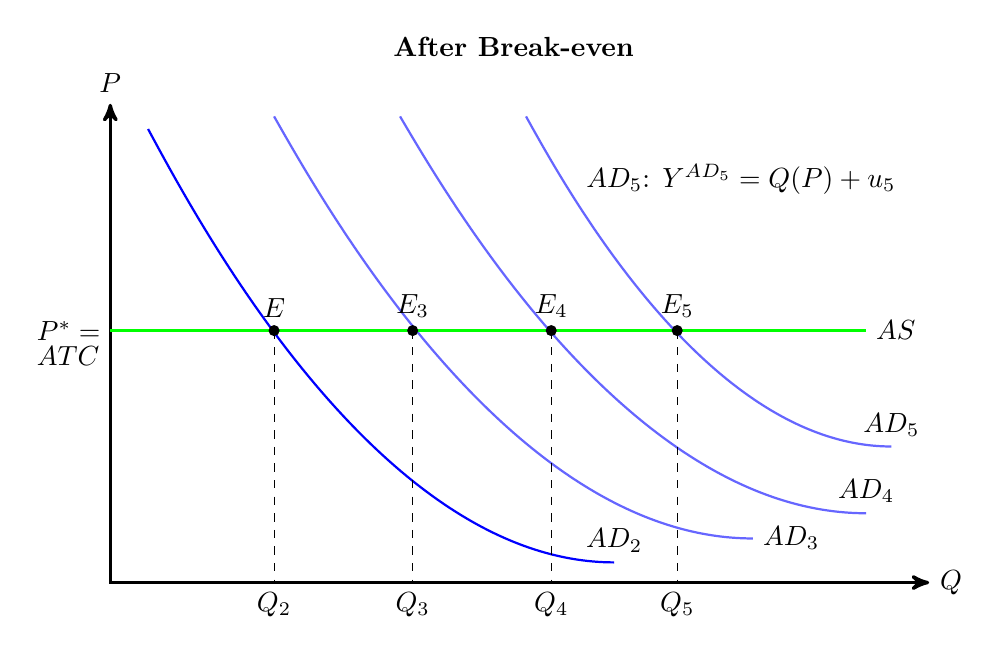
\begin{tikzpicture}[
        scale=1.6,
        IS/.style={blue, thick},
        LM/.style={red, thick},
        axis/.style={very thick, ->, >=stealth', line join=miter},
        important line/.style={thick}, dashed line/.style={dashed, thin},
        every node/.style={color=black},
        dot/.style={circle,fill=black,minimum size=4pt,inner sep=0pt,
            outer sep=-1pt},
    ]

    \draw[axis,<->] (6.5,0) node(xline)[right] {$Q$} -|
                    (0,3.8) 
                    node(yline)[above] {$P$};

    \draw[IS] (0.3,3.6) coordinate (IS_1) parabola[bend at end]
         (4,0.16) coordinate (IS_2) node[above] {$AD_2$};

    \draw[xshift=1cm, yshift=.1cm, IS, blue!60] (0.3,3.6)
        parabola[bend at end]  (4.1,0.25)
        node[right] {$AD_3$};

    \draw[xshift=2cm, yshift=.1cm, IS, blue!60] (0.3,3.6)
        parabola[bend at end]  (4,0.45)
        node[above] {$AD_4$};

    \draw[xshift=3cm, yshift=.1cm, IS, blue!60] (0.3,3.6)
        parabola[bend at end]  (3.2,0.98)
        node[above] {$AD_5$};
        
    \draw [important line, green] (0,2) -- (6,2);


    \coordinate[label= right:{$P^*=$}] (p) at (-0.66,2) ; 
    \coordinate[label= right:{$ATC$}] (atc) at (-0.66,1.8) ; 
    \coordinate[label= right:{$AS$}] (as) at (6,2) ; 

    \coordinate[label= below:{$Q_2$}] (q0) at (1.3,0) ; 
    \coordinate[label= below:{$Q_3$}] (q1) at (2.4,0) ; 
    \coordinate[label= below:{$Q_4$}] (q2) at (3.5,0) ; 
    \coordinate[label= below:{$Q_5$}] (q2) at (4.5,0) ; 

    \node[dot,label=above:$E$] at (1.3,2) (int1) {};
    \node[dot,label=above:$E_3$] at (2.4,2) (int2) {};
    \node[dot,label=above:$E_4$] at (3.5,2) (int3) {};
    \node[dot,label=above:$E_5$] at (4.5,2) (int3) {};

    \draw [dashed] (1.3,2) -- (1.3,0);
    \draw [dashed] (2.4,2) -- (2.4,0);    
    \draw [dashed] (3.5,2) -- (3.5,0);    
    \draw [dashed] (4.5,2) -- (4.5,0);    

    \coordinate[label= right:{$AD_5$: $Y^{AD_5}=Q(P)+u_5$}] (q2) at (3.7,3.2) ; 
        
    \coordinate[label= above:\bf{After Break-even}] (p5) at (3.2,4.1);
   
\end{tikzpicture}

Growth in $u$ will shift $AD$ curve further and further outwards that will increase the equilibrium quantity of CENTRAPAY. For instance, when $u$ increases to $u_5$, the equilibrium quantity of CENTRAPAY increases to $Q_5$. Note that this larger quantity of CENTRAPAY indicates more network usage, which increase the demand for CENNZ. 

\section{Incentives of Validators}
Although expected return of CENTRAPAY is zero by model design, all validators are CENNZ stakers that they all benefit from positive expected demand of CENNZ as network usages grow.   \par

For a risk-neutral validator, 
$$Expected Return=ER[CENTRAPAY]+ER[CENNZ]>0$$

For a large stake holder, as long as the return is high enough, he/she is willing to accept the initial lower price at the bootstrapping periods,
$$Expected Return=Initial Loss+ER[CENTRAPAY]+ER[CENNZ]>0$$

For a risk-taking validator, who values future demand for CENNZ more, as long as this part of expected utility is large enough, he/she is willing to accept the initial lower price at the bootstrapping periods,
$$Expected Utlity=EU[Initial Loss]+EU[CENTRAPAY]+EU[CENNZ]>0$$

\section{Conclusion}
By setting Mint Multiplier strategically, having some large stake holding validators and/or risk-taking validators willing to supply CENTRAPAY at lower prices in early stages, promoting network usage well enough to boost aggregate demand, we will be able to build a sustainable network, in which value of CENTRAPAY is stabilized in terms of purchasing powers, at a market price that equals to its cost of production, and the growth of the network will raise the demand for CENNZ.\par

While promoting network usage in bootstrapping periods is essential to the success of our model, it is mostly about boosting demand through exogenous price-independent factors, e.g. getting more popular dApps adopting our network. \par

The concept of our unique unit of measurement, Current CPU Cost ($CCC$) that we use to value all costs, market prices and returns, is a valuable contribution to the industry, which is a truly decentralized solution independent of centralized information. We not only do not need to worry about changes in purchasing price of CPU and storage elements via fiat currency in real life, values measured in $CCC$ provides all our users, especially companies an excellent guideline on cost budgeting and return estimation of adopting our network, a critical factor in understanding which infrastructure to build an application on. 


\section{Discussion}
Estimations about the first break-even point can be calculated by estimating market demand using live data after launch, or a brief estimate can be drawn by analyzing empirical evidences of other cryptocurrency network with similar nature. \par

The model can be extended further to capture future changes, including a different reward system that validators are rewarded according to properties of their stakes or nodes, users offer to pay a markup in transaction fee to get their transactions processed faster at peak time when our network becomes super busy reaching full capacity. 

\end{document}